\documentclass[border=10pt]{standalone}

\usepackage{pgfplots,siunitx}
\pgfplotsset{compat=newest}

\def\kB{1.38e-23} % Boltzmann constant
\def\mu{6.64e-27} % unified atomic mass unit/Dalton (symbols: m_u or Da)

\def\maxwellboltzmann#1{1000* 4 * pi * (\mu / (2 * pi * \kB * #1))^(3/2) * x^2 * exp(-\mu * x^2 / (2 * \kB * #1))}

\begin{document}

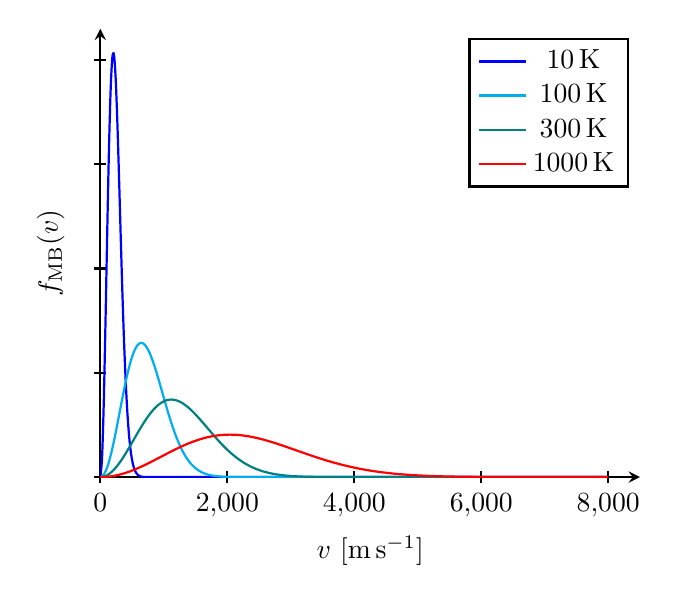
\begin{tikzpicture}

  \begin{axis}[
      domain = 0:8000,
      xmin = 0,
      xmax = 8500,
      ymin = 0,
      ymax = 4.3,
      xlabel = {$v$ [\si{\metre\per\second}]},
      ylabel = $f_\text{MB}(v)$,
      yticklabels=\empty,
      smooth, thick,
      axis lines = left,
      every tick/.style = {thick},
    ]
    
    \addplot[color=blue, domain=0:8000, samples=300]{\maxwellboltzmann{10}};

    \addplot[color=cyan, domain=0:8000, samples=300]{\maxwellboltzmann{100}};

    \addplot[color=teal, domain=0:8000, samples=300]{\maxwellboltzmann{300}};

    \addplot[color=red, domain=0:8000, samples=300]{\maxwellboltzmann{1000}};

    \legend{\SI{10}{\kelvin}, \SI{100}{\kelvin}, \SI{300}{\kelvin}, \SI{1000}{\kelvin}};

  \end{axis}
\end{tikzpicture}

\end{document}